\documentclass[12pt, a4paper]{report}
\usepackage[utf8]{inputenc}
\usepackage[english]{babel}
\usepackage{amsmath}
\usepackage{minted}
\usepackage{dirtree}
\usepackage{palatino}
\usepackage{syntax}
\usepackage{geometry}
\usepackage[hidelinks]{hyperref}
\usepackage{graphicx}
\usepackage{sidecap}
\usepackage{tikz}
\usetikzlibrary{matrix}
\usepackage{cite}
\usepackage{color, colortbl}
\definecolor{Seagreen}{rgb}{0.18, 0.54, 0.34}
\definecolor{Lawngreen}{rgb}{0.48, 0.99, 0}
\definecolor{LRed}{rgb}{1, 0.8, 0.8}
\definecolor{GoldenRod}{rgb}{0.93, 0.65, 0.12}
\usepackage[center]{titlesec}
\linespread{1.3}
\usepackage{verbatimbox}

\setlength{\parindent}{0pt}
\setlength{\parskip}{1em}

\begin{document}
\begin{titlepage}
    \centering
    %% \includegraphics[width=0.15\textwidth]{example-image-1x1}\par\vspace{1cm}
    {\scshape\LARGE University College London\par}
    \vspace{1cm}
    {\scshape\Large MSc Computer Science}
    \vspace{1.5cm}
    {\huge\bfseries MicroML \\ A Functional Programming Language for the BBC micro:bit \par}
    \vspace{2cm}
    {\huge\itshape David Kelly\par}
    \vfill
    supervised by\par
    {\large Rae \textsc{Harbird}}

    \vfill
    {\large \today\par}

    \vfill

    This report is submitted as part requirement for the MSc Computer Science
    degree at UCL\. It is substantially the result of my own work except where 
    explicitly indicated in the text.
    
    \vfill

    The report may be freely copied and distributed provided the source is explicitly
    acknowledged.
\end{titlepage}

\tableofcontents
\newpage

\begin{abstract}
It is increasingly being recognized in educational circles that introductory lessons in programming
are a vital part of the modern school curriculum. Programming education in UK has not traditionally
formed a central part of the syllabus. Nearly all teenagers have access to computers and devices, but very
few know how to program them themselves. The raspberry pi has seen a remarkable growth in
popularity since its introduction a mere four years ago. The BBC micro:bit is a project in the
same spirit as the raspberry pi, but with a remit specifically for UK secondary school students.

MicroML is an attempt to bring the fundamental concepts of the functional programming paradigm
to the micro:bit, and thusly to the large body of untapped talent lying in Britain's secondary
schools. It should allow the students to explore such ideas as recursive thinking, structural
induction, polymorphism and higher order types without ever having to be exposed to the
underlying theory of such things, something which no other functional language does.  

The project was conceived and written in Haskell. It does not build on any other existing
project. Apart from reliance on standard Haskell libraries all of the major design work was
written `ab nihilo', including syntax design, the parser, type inference, repl and compiler.  

MicroML, at point of submission, is a strong base from which to do further work. It has
polymetric type inference, markdown-style inline documentation, a fully-featured repl
environment with extensive error checking capabilities, the ability to check source code for
common programming errors (such as duplicate function definitions and unreachable functions) and
produce images of program callgraphs. It has been designed with the principle aim of making an
environment conducive to learning, without being condescending or overly simplistic. 

\end{abstract}
\chapter{Introduction}

\begin{flushright} \textit{`a monad is a monoid in the category of endofunctors, what's
the problem?'} \\ --- not Philip Wadler\footnote{The quote is actually from \textit{A
Brief, Incomplete, and Mostly Wrong History of Programming Languages by James Iry
\url{https://james-iry.blogspot.co.uk/2009/05/brief-incomplete-and-mostly-wrong.html}}, where it is
deliberately falsely attributed, but it is itself a close paraphrase from \textit{Categories for the
Working Mathematician}.} 
\end{flushright}

\section{Motivation} 
The Wadler quote might be spurious, but a genuine piece of
documentation drawn from the Control.Monad.Trans.EitherT
library\footnote{\url{https://hackage.haskell.org/package/either-4.4.1.1/docs/Control-Monad-Trans-Ei
ther.html}} available from \textit{Hackage} informs us that `an apomorphism is the generalized
anamorphism for this Monad'. Such statements, while (almost certainly) factually correct are of
little use to the average `jobbing' programmer and indeed must be considered to have the effect
of deliberately alienating a large part of the software engineering workforce. One can only hope
that this was not the intention, because functional languages, especially those which use static
type analysis and inference, have a great deal to offer to the programming community in terms
of expressiveness and safety. Must it be the case therefore that introductory material is so
intimidating? Is there a way to encourage students to think functionally, in a type-orientated
manner, without the heavy mathematical `baggage' that is simply surplus to requirements when writing
one's first programs?

\section{Aims and Goals}
\subsection{Project Aims}
It seems only apposite that a functional language for the micro:bit, assuming that it is not
self-hosting, should be written in a more mature functional language. Haskell was chosen for this
task as it presented a good opportunity to `come to grips' with the language and the paradigm. A
single 10-week module in Miranda was not, as anticipated, sufficient preparation for the complexity
of constructing an entire program in a language which is almost aggressive in its focus on purity. 

The primary target, or goal, of the project is to produce, as a first iteration, the basis of a
language designed primarily for teaching purposes, but practical enough to write real programs for
the micro:bit. Many languages have been implemented over the years with the express aim of teaching
programming concepts. Perhaps the most famous and successful of these is Scheme. However, what they
all have in common is that they are intended for an audience who are already interested in computer
science, or are indeed computer scientists. Even classic texts, such as \textit{The Implementation
and Interpretation of Computer Programming} is squarely pitched at a sophisticated audience.
The micro:bit is the opposite: it is for students with no previous programming experience,
students who are not mathematicians, teachers who are neither mathematicians nor programmers.
Functional programming has a reputation in the programming community as being complex and only for a
special type of person. The aim of this project is to show that this is not necessarily be the case.
With this in mind, the aim is to make the language as education as possible, at the expense of
sacrificing expressiveness. 

% Mention here no call with current continuation or macros, as obscuring underlying goals, which are
% inductive reasoning and intro to types and function composition.

Development progressed iteratively. Having no previous experience of engineering a large software
project in Haskell, initial development was largely \textit{ad hoc} and unstructured. Haskell is not
an ideal language for development in this manner. A great deal of time was spent just in understanding 
the principles of state manipulation in a side-effect free language. Luckily there were a number of 
tutorials which served as the backbone, or perhaps more accurately, embryo, of the final project. 
Traces of these tutorials can still be seen scattered throughout the final codebase. These were 
perhaps both a help and a hindrance, as their original authors had not perhaps foreseen that 
they would be so heavily expanded and built-upon. Strong foundations might have results in a project 
which was more realised, with fewer edge cases and areas where the solutions are not as robust as could be desired. \\

\subsection{Project Goals}
Formally put, the project's goals in order of importance are 

\begin{itemize}
    \item Create an uncluttered syntax for a functional language. The initial inspiration was a
        mixture of Scheme and Miranda. Scheme was considered the better model for evaluation (but
        not for syntax) as it is very simple and relatively pure. While Scheme lacks such items as algebraic data types
        and pattern matching, it clearly exposes the underlying lambda calculus.
    \item Write a repl environment for students to explore code and concepts. All modern languages
        ought to have a repl, so that individual snippets of code can be tested without the delay of
        compilation and the increased difficulty of pinpointing errors. The repl environment ought
        to be `friendly' and provide as much assistance to the user as possible. 
    \item Have effective type inference so that students do not need to explicitly type variables.
        While not every functional language has type inference\footnote{Idris, a dependently typed language,
            requires type annotations due to the undecidability of inference of dependent types.},
        it is a fundamental feature of the ML family. Having type inference means that the `truth'
        of types is not hidden from the student as it would be with JavaScript or Python, but the
        onus of type annotations is also absent.
    \item Compiler to micro:bit flavoured C++. This part of the project which was most
        pertinent to the micro:bit, but also that which would require the most time to bring to a
        degree where compilation of even complicated programs could be accomplished with safety and
        precision. 
\end{itemize}

\chapter{Context} 
\section{The BBC micro:bit} The BBC micro:bit is a microprocessor device aimed at
bringing programming to young adults and teenagers. At present it supports a number of different
programming languages, most visibly \textit{MicroPython, JavaScript} and \textit{TouchDevelop}.
These languages, while mainstream and popular,\footnote{With the exception of \textit{TouchDevelop}
of course.} all fundamentally support the same programming paradigm, the imperative. Doubtless it
is vital for all would-be coders to have knowledge and experience with the imperative/procedural
approach to structuring code, but it is not the only approach, and perhaps not the best for
beginners or those with only a passing interest in coding. It is the contention of the author that
a syntactically simple, (relatively) \textit{pure} functional language would make for an ideal
teaching tool on the micro:bit, allowing the student to focus almost entirely on the problem domain,
and a great deal less on syntax and \textit{boilerplate}. Functional languages are increasingly
being used in every area of real-world applications. Regarding robotics, in which Rae has expressed
an interest, there has already been some research conducted in the use of the declarative style
for low level robotics programming\footnote{Lambda in Motion: Controlling Robots with Haskell,
Peterson John, Paul Hudak and Conal Elliott}. This at least demonstrates that the functional style
is applicable to the problem area, but further research would be required to test the suitability of
the micro:bit as a low-level controller. Certainly, anything which can be programmed in MicroPython
could also be written (possible more briefly and with fewer bugs) in a functional language.

\section{Teaching Languages}
There is a long history of languages designed with the express purpose of teaching rather than
production. These generally fall into two streams of development: reduced versions of established
professional languages, and graphical environments. In general, the visual programming languages, of
which \textit{Scratch} is undoubtedly the most well established, are intended for a younger age
group. On the micro:bit \textit{Microsoft Block Editor} is of this variety. 
\textit{Microsoft Touch Develop} and \textit{Code Kingdoms JavaScript} appear to offer a hybrid
experience, with textual code presented in a coloured, graphical editor. Finally there is a port of
the \textit{Python} programming language, which best typifies that school of tuition where a real
language is used in a simplified context.

\section{Python as Teaching Language}
While Python was not explicitly designed as a teaching language, in recent years it has increasingly
been used as an introductory language in university settings. MIT, where Scheme was first created
and promoted, has begun to teach its introductory courses in Python. With Python already available
on the micro:bit, why is there the need for another text-based language on the same platform? Is
this not just `muddying the waters' of what should be a simple educational tool. Do instructors
really have the time to learn another language if students should express an interest in programming
functionally?


\section{Python vs Miranda/Haskell}
In an attempt to address some of these questions, it is necessary to derive some picture of what might
constitute a functional language, and why it might be a useful way to teach programming to younger
learners. Being more a philosophical stance than technical necessity, it is possible to mix various
paradigms together to form \textit{hybrid} languages. In practice, most programming languages take
precisely this approach\footnote{Truly pure languages are a rare thing: in the realms of OOP perhaps
only \textit{Smalltalk} and \textit{Ruby} qualify. In the functional language family, the only
mainstream entirely pure language is Haskell.}. Python, for example, supports a great deal of the 
functional paradigm, as does JavaScript. These already exist on the micro:bit: why not just use those? 
Consider the following simple scenario, we want to sum all the occurrences of the number 3 in the
following list: 

\mint{python}|nums = [2,3,4,3,2,3,5]|

To do this in an imperative manner, something like the following might be written:

\begin{minted}{python}
    sum = 0
    for i in range(len(nums)):
        if nums[i] == 3:
        sum += 3
\end{minted}

To solve this in Python using functional concepts, something like this might be used:

\mint{python}|sum(list(filter((lambda x: x == 3), nums)))|

This is clearly an improvement in terms of brevity, and is perhaps a little easier to understand.
The main difficulty here in the physical writing of the code is balancing the parentheses,
but any good editor should be able to do this automatically. The filter higher order function
\textit{filter} has a fairly clear meaning to any native English speaker. However the rather obscure
use of \textit{list} and, even worse, \textit{lambda} still makes this rather difficult for the
student. There is a number of topics which would need to be explained here which reduce the utility
of this as a teaching example. Why is the syntax still relatively cumbersome? Because Python was
not conceived as a functional language, many of these features have been grafted onto a traditional
imperative substructure, and the syntax reveals this. The equivalent function in Haskell would be:

\mint{haskell}|sum (filter (==3) nums)|

Haskell provides some syntactic sugar to reduce the number of brackets even
further\footnote{Apologies for the slightly misleading typography here, the package being used for
syntax highlighting seems unable to properly interpret \LaTeX escape symbols. It should read simply
\$.}

\mint{haskell}|sum \$ filter (==3) nums|    
To make all of this code more generic the Python needs to be wrapped in a function definition:

\begin{minted}{python}
    def sumAllOccurrences(n, nums):
        sum = 0
        for i in range(len(nums)):
            if nums[i] == n:
                sum += n
        return sum
\end{minted}

And the equivalent in Haskell:

\mint{haskell}|sumAllOccurrences n ns = sum \$ filter (==n) ns|

In fact, we can do even better than this:

\mint{haskell}|sumAllOccurrences p ns = sum \$ filter p ns|

where p is any predicate we care to pass in, such as (==3) or (\textless2). The python code does not
prevent someone from passing in junk values (leading to a runtime error) but the Haskell code, with
the addition of a simple \textit{type signature} can easily be altered to only receive integers,
ensuring type safety. This need not be explained to the student in these terms, but they will
benefit from their program not crashing in unexpected and difficult to detect ways.

\begin{minted}{haskell}
    sumAllOccurrences :: (Int -> Bool) -> [Int] -> Int
    sumAllOccurrences p ns = sum \$ filter p ns
\end{minted}

This is more powerful than the equivalent Python for loop definition, and a great deal more
flexible. Obviously this could also be implemented in python using filters and lambda expressions,
but it would still need to be couched inside a function definition.\footnote{This is slightly
disingenuous, as a list comprehension, in both Python and Haskell, would work well here. It does
serve to illustrate the general point. Of course, list comprehensions were first introduced in
functional programming languages.}. In this simple example much of the essence of the functional
programming style can be seen. The advantages are clear: fewer lines of code usually means fewer
bugs and less development time. Students can get to solving problems almost immediately, without the
worry (or rather a reduced worry) about the syntactical correctness of their loops, or balancing
a host of nested parentheses. %Haskell is a large and complicated language and not suitable for
younger students\footnote{make a reference here or somewhere to the eitherT library, by Kmett}.
Its runtime is large and complex, and would almost certainly not run efficiently on the micro:bit.
Its emphasis on purity has led it to introduce a number of features which, while theoretically
elegant, are complex even for experienced programmers. There is however a family of other, related,
languages, mostly descended directly or indirectly from ML\footnote{Excepting the Lisp family
representatives, \textit{Common Lisp} and \textit{Scheme}}, which place different emphasis on parts
of the functional paradigm.\footnote{The table is a simplified (and slight corrected) version of the
available from \url{https://en.wikipedia.org/wiki/Comparison_of_functional_programming_languages}.
Monads, monoids and functors, while important concepts in functional languages, are definitely out
of scope for a teaching language to teenagers. The approach taken by \textit{Miranda} is that which
will be followed in the suggested implementation, hiding unnecessary detail with the loss of a
little referential transparency.}

\section{Research}
With the thought in mind of creating a Miranda style language for the micro:bit, came the necessity
to decide on the technologies and theoretical basis for the language. Being an implementation of the
lambda calculus, it was necessary to choose an axis on the \textit{lambda cube} for further
development. 

\subsection{The Lambda Cube}
The Lambda Cube was introduced by mathematician Henk Barendregt as a visualization framework for
Coquand's calculus of constructions. The simple untyped lambda calculus is not
represented.\footnote{Pierce p.465 has a slightly different treatment of the axes.}


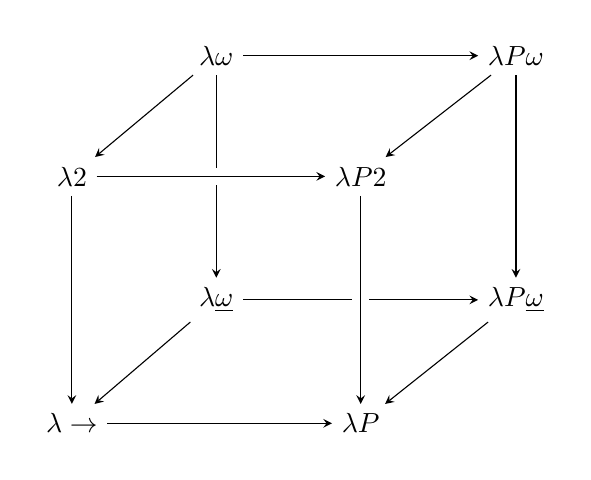
\begin{tikzpicture}
  \matrix (m) [matrix of math nodes, row sep=3em,
    column sep=3em]{
        & \lambda\omega & & \lambda P \omega \\
        \lambda 2 & & \lambda P 2 & \\
        & \lambda \underline{\omega} & & \lambda P \underline{\omega} \\
        \lambda \rightarrow & & \lambda P  & \\};
  \path[-stealth]
    (m-1-2) edge (m-1-4) edge (m-2-1) edge (m-3-2)
    (m-1-4) edge (m-3-4) edge (m-2-3)
    (m-2-1) edge [-,line width=6pt,draw=white] (m-2-3)
            edge (m-2-3) edge (m-4-1)
    (m-3-2) edge (m-3-4)
            edge (m-4-1)
    (m-4-1) edge (m-4-3)
    (m-3-4) edge (m-4-3)
    (m-2-3) edge [-,line width=6pt,draw=white] (m-4-3)
            edge (m-4-3);
\end{tikzpicture}

This can be understood as a exploring refinements of of type lambda calculi. Starting in the bottom
left hand corner $\lambda \rightarrow$ is the simply type lambda calculus as developed by Church,
Curry and Feys in the 1940s\footnote{Types and Programming Languages p11 gives a simple timeline of
    type theory research.}. The top right corner, the `summit' of calculi is $\lambda P \omega$, which
represents dependent types. Perhaps no truly practical programming language occupies this space at
present. Theorem provers, such as \textit{Coq} have not been used for enterprise software, and
perhaps it is not possible to do so. \textit{Idris}, a dependently typed programming language
written in Haskell, is an attempt to write a general programming language with dependent types. It is
too early in its development at this stage to say whether it will meet with success. A number of
issues, principally the undecidability of type inference over dependent types, would seem to be a
limiting factor to general acceptance. 

Naturally, microML makes no attempt to implement $\lambda P\omega$. `Real world' functional
languages, such as Haskell, actually implement hybrid systems which are not represented on the cube.
Most importantly, subtyping (represented as $\lambda F_{<:}$) is missing as a construct from the cube, 
even though almost all language which support record syntax must allow some form of subtyping.

$\lambda 2$, or \textit{System F} is that system which allows for parametric polymorphism (often
called \textit{generics} in such languages as Java and C++). This seemed a suitable target for
microML's type system. It has the added advantage that there is a well-established algorithm, Damas
--- Milner algorithm W, which runs in $\mathcal{O}(n)$ time for non-pathological input\footnote{Worst case
    complexity for algorithm W actually falls into exponential time, but an input program would have
    to be both perversely written and extremely large before this would become a significant
    liability.}. Type inference was deemed an important addition to microML as introducing the
concept of types, which though fundamental to modern computing, carries the risk of rendering it too
difficult and different conceptually from the other languages already available on the micro:bit.
These all have in common so-called \textit{duck} typing, and interaction with the type system,
programming with types as it were, is against the nature of the language itself. This is especially
true of Python, which discourages direct type checking on the part of the programmer (though such
facilities do exist.). Good type inference, with easy to read error messages, is an essential
feature of microML without which it would struggle to justify its existence.

\section{Sources}
This project has drawn on a large variety of sources, some only tangentally, but others central to
the realization of the project, without which microML, as embryonic as it might be, would not exist
at all. A number of tutorials (detailed in the bibilography) gave a strong starting position upon
which to build. Luckily there are a number of trivial examples of repls written in Haskell which
give an idea of what might be accomplished. Full scale compilers are a little more unusual, but such
classic texts as `Modern Compiler Implementation in Standard ML', the so-called \textit{Tiger Book},
can be adapted to Haskell with minimal inconvenience. For type theory the central text is
undoubtedly `Types and Programming Languages' without which many a tutorial on type inference would
have remained decidedly opaque.

Many papers were consulted initially while deciding on the best approach for microML's type system.
In practice, very little of this reading has made it into the language as currently constituted, but
it is hoped that the design allows for future development to integrate some of these possible
features easily. Always bearing in mind of course the intended scope of the language. This perhaps
was one of the most difficult design decisions: what had a legitimate place in a language for a
simple processor aimed at teachers, and what could be implemented simply for the interests of the
developer, or because it was simple to do? Design decisions based on ease of implementation or to
please the vanity of the designer are correct only be coincidence, and this is a poor way to
design\footnote{This recalls Tony Hoare's `Billion Dollar Mistake'.}.

\section{Software, Tools, Libraries}
Haskell is ideally suited to the creation of DSLs. This is largely due to its \textit{algebraic data
    types} which can easily be used to represent the BNF of an embedded language. Moreover Haskell is
blessed with the Parsec library of parser combinators\footnote{A \textit{combinator} is simply a
    function with no free variables, so it only operates on parameters directly passed to it without
    reference to any global data within the function body.}, which mitigates against the necessity of
writing lex and yacc files to create a functioning parser. A parser for another language can be
implemented directly in Haskell, using standard Haskell syntax. Haskell moreover has an extensive
library system, located on \textit{Hackage}. There is a library for almost any conceivable
requirement. Haskell has two main build tools for project management. Neither is as tightly
integrated into the language as might be ideal. One need only compare newer languages, such as Rust
and Elixir, where the build tools (Cargo and Mix in this case) are an integral part of the language,
to realize that both \textit{Cabal} and \textit{Stack} have a rather \textit{grafted on} aspect.

All Hackage packages are available through Cabal, but version management is not rigorously
enforced. Builds can break easily and frequently. So-called `Cabal dependency
Hell'\footnote{\url{https://wiki.haskell.org/Cabal/Survival}} is a real problem, especially for
those with no prior experience with the tool. It is poor design to inflict such problems on an end
user who only wants to build a piece of software from source rather then having the programmer
subsume them. Stack helps in this direction but maintaining a stable list of packages and creating a
strong sandboxed environment for development. The price to be paid is a reduced number of available
libraries, so build problems can still occur over external dependencies. MicroML was firstly a Cabal
project, but was migrated to Stack later in development. This largely produced a more stable
build and allowed for the use of \textit{intero}\footnote{intero is an alternative to ghci --- the
    Haskell interactive environment, but provides better type information and error messages,
    moreover it has good integration with neovim, the author's editor of choice.} but unfortunately also meant that some experimental
code (specially the JIT compiler) had to be disabled. This will be discussed more fully in chapter
<unknown>.

Some libraries and approaches were abandoned during the development process. Most notably a deal of
time was put into using the \textit{Language-C} library for manipulating the C AST in Haskell. While
this would certainly be the correct approach for writing the C code generation element of microML,
it was decided that time constraints did not allow for proper utilization of the library (which is
very large) so other alternatives were explored in the hope of at least producing a testable backend
within the time frame of the project. 

\chapter{Requirements and Analysis}

If the task is to design and implement a functional programming language, the obvious question is: What is a functional language? 
Examining some of the leading languages widely regarded as belonging to the family, a number of
features emerge.

\begin{center}
\addvbuffer[20pt 20pt]
{\begin{tabular}{|c|cccccc|}
    \hline
                & Pure                    & Lazy Evaluation     & Typing                      & Algebraic Data Types     & Immutable Data          & Closures \\
    \hline
    Common Lisp & No                      & \cellcolor{LRed}Yes & Dynamic                     & \cellcolor{GoldenRod}Yes & No                      & \cellcolor{LRed}Yes \\
    Scheme      & No                      & No                  & Dynamic                     & No                       & No                      & \cellcolor{LRed}Yes \\
    ML          & No                      & No                  & \cellcolor{Lawngreen}Static & \cellcolor{GoldenRod}Yes & No                      & \cellcolor{LRed}Yes \\
    F\#         & No                      & \cellcolor{LRed}Yes & \cellcolor{Lawngreen}Static & \cellcolor{GoldenRod}Yes & No                      & \cellcolor{LRed}Yes \\
    Clojure     & No                      & \cellcolor{LRed}Yes & Dynamic                     & \cellcolor{GoldenRod}Yes & \cellcolor{Seagreen}Yes & \cellcolor{LRed}Yes \\
    Miranda     & \cellcolor{Seagreen}Yes & \cellcolor{LRed}Yes & \cellcolor{Lawngreen}Static & \cellcolor{GoldenRod}Yes & \cellcolor{Seagreen}Yes & \cellcolor{LRed}Yes \\
    Haskell     & \cellcolor{Seagreen}Yes & \cellcolor{LRed}Yes & \cellcolor{Lawngreen}Static & \cellcolor{GoldenRod}Yes & \cellcolor{Seagreen}Yes & \cellcolor{LRed}Yes \\
    \hline
\end{tabular}}
\end{center}

\textit{Purity} is a rather vexed term than has seen a great deal of discussion in the literature
and on such websites as \textit{reddit}. For the purposes of the following discussion, purity will
be considered the ability to write equational code within an impure framework. A Haskell program,
for example, lives within the IO monad. The IO monad is necessarily impure, as it involves
interacting with a system (in this case the operating system) where such interactions are not
predicated on input data. However, on the assumption that the operating system will perform the
actions requested of it, the code running \textit{inside} the IO monad can be understood as
completely referentially transparent. That is, a function called with the same arguments will always
return the same results. This is not necessarily the case with a language like Scheme, which as the
`set!' operator for manipulating global state in a non-transparent manner. 

The table shows clearly that there are a few central features which are associated with functional
languages, and other features which are less essential. Bearing in mind the target audience and the
target device, is should be fairly safe to abandon explicit monads and monoids. Higher order functions are
essential to the paradigm, as is partial function application.\footnote{i.e.\ allowing functions to
    accept fewer arguments than their arity would suggest. The classic example is \mint{haskell}|inc = (+1)| where
    the + operator has been partially applied.}

Algebraic data types (ADTs) are found in nearly all of the major functional languages. The notable
exception again is Scheme. This is of additional interest in that Scheme is the only Language of
those listed which was explicitly designed as a teaching language. It is worth clarifying at this
stage that any complete lambda calculus implementation has the potential to create ADTs, the missing
element is the syntactic sugar provided the sum and product types in languages such as ML and
Haskell. The same is also true of tuples and lists, which do not require special status in a
lambda calculus language, but are often given so for reasons of efficiency and programmer
satisfaction. The immediate application of ADTS for  micro:bit programming is not immediately
apparent, so, much in the manner of Scheme, these will not be considered a priority of microML.

\section{Requirements \& Constraints: Language Design}
Miranda\textsuperscript{TM} is a language created by David Turner in the early 1980s\footnote{The wikipedia 
    page says that Miranda supports monads. This is not correct, in
    the sense that it is not possible for the programmer to create monad instances or explicitly
    interact with monads. It is also
unlikely that Miranda is using monadic concepts at the implementation level as these were first
introduced into Haskell a number of years after the introduction of Miranda}. It is a member
of the ML family, one of the first purely functional programming languages, and the direct parent of
Haskell and Haskell's various offshoots. Indeed, one of the reasons for the creation of Haskell was
the fact that Miranda was trademarked and closed source. It might best be described as a (small)
subset of Haskell\footnote{Though it would be more accurate to describe Haskell as a superset of
    Miranda.}. It is still used as a teaching language and has a very clean, simply syntax. A
reduced version of Miranda is suggested for the language, which will go under the working title of
microML.\footnote{microMiranda would probably be a more honest name, but there might be a small
    risk of copyright infringement.}

Miranda has an reasonably rich standard library, which comes automatically with the interpreter. MicroML
should have a subset of this standard library, with functions such as map, filter and fold\footnote{Miranda 
    distinguishes between left and right folds. This, while very flexible, might be
too complex for most students. Both Clojure and Python have a simple \textit{reduce} which has the
behaviour of a right fold. In Clojure \textit{apply} is similar to a left fold.}. As far as possible, 
all built-in functions should be \textit{safe}, that is, there should be no
partial functions in the standard library. A partial function is one which does not produce a legal
result for every legal input, for example taking the head of an empty list in Haskell or Miranda
results in a error.

\begin{minted}{haskell}
    head []
    *** Exception: Prelude.head: empty list
\end{minted} 

However this is not a necessity\footnote{The head function in Haskell's standard prelude is a legacy
    from Miranda which unfortunately is too late to change easily. The Idris language (itself
    written in Haskell) has a built-in function totality checker, usable from the repl, to ensure
that such unsafe practices are deliberate rather than accidental or due to programmer laziness.} 
and safe versions of these functions should be written for microML. 

Laziness, or more accurately non-strictness,  is an interesting feature of many functional languages, 
but it is a little unclear at the moment what this would mean for programming on the micro:bit. 
Laziness is chiefly useful when dealing with infinite data structures, which is an unlikely
scenario. Moreover, lazy evaluation can make reasoning about the structure of a program more
difficult than is necessary at this stage of the programmer's development, where a more literal
`first this then this' might be easier to understand. 

Another of the more interesting features of the ML family is type inference and static typing. This
is unlikely to be of huge interest to the average student, but it has many benefits. Most
importantly, errors which in a language like Python would only be caught at runtime do not get past
the compilation stage of an ML-style language. Student-friendly (rather than detailed
programmer-friendly) error messages will have to be
written to help the student understand what they have done wrong. Type inference should limit the
student's direct interaction with the type system, which can be very difficult to understand.

Every functional language has algebraic data types. They are fundamental to how any large program is
constructed. They can be used to simulate enumerations in other languages and as value constructors
(vital in constructing ASTs for example). With regard to the field of robotics for example, to
should be possible to create ADTs which describe the behaviour and attributes of the robot.

Immutability of data is a key (but not universal) feature of the functional paradigm. It allows for
referential transparency and an easier approach to concurrency. Again, these are not features which
are vital to the micro:bit, but they will help students in the future who wish to continue their
coding. Indeed, immutability is in many ways more intuitive for students. If x = 6, then it is 6 for
the entire program. This is a much simpler concept than having a value for x which can go up and down,
or even change type.


\chapter{Design and Implementation}

\subsection{Design}
microML uses an enriched lambda calculus as its base
\vspace{5mm}

\begin{minipage}[t]{0.5\textwidth}
    \begin{grammar}
        <Expr> ::= Var
        \alt{} Constructor 
        \alt{} Application <Expr> <Expr>
        \alt{} Let Name <Expr> <Expr>
        \alt{} Literal 
        \alt{} If <Expr> then <Expr> else <Expr>
        \alt{} FixPoint <Expr>
        \alt{} UnaryOp <Expr>
        \alt{} BinOp <Expr> <Expr>
        \alt{} PrimitiveErr 
        \alt{} Nil
    \end{grammar}
\end{minipage}
\begin{minipage}[t]{0.5\textwidth}
    \begin{grammar}
        <Literal> ::= Integer
        \alt{} Double
        \alt{} Boolean
        \alt{} String
        \alt{} Char
        \alt{} Tuple of <Literal>
    \end{grammar}
\end{minipage}
\vspace{5mm}

It will be observed that two number formats are supported in the parse tree, integers (which in
Haskell are unbounded big numbers) and doubles. The type system however only recognizes a
generalized \textbf{Number}. This decision will be discussed more fully in Section~\ref{sec:type}.

In addition to these basic primitives and control structures, microML also makes use of three
primitives inherited from languages in the Lisp family:

\begin{grammar}
    <UnaryOp> ::= Car
    \alt{} Cdr
    \alt{} Cons
    \alt{} Show
    \alt{} Read
\end{grammar}

These primitives are accessed through the \textit{head}, \textit{tail} and (:) built-in functions and are
essential for recursing over lists.\

MicroML, in addition to floats and ints, also supports binary, octal and hex numbers\footnote{The
    syntax for these is inspired by erlang, one simply writes the number in the form e.g.\ 2\#110 for a
    binary 6. Likewise octal is 8\# and hex 16\#}. These are not
treated as primitives however, and are automatically converted to an appropriate numeric representation.

The \textit{FixPoint} primitive allows for the creation of recursive functions by satisfying the equation
\begin{flalign*}
    &y\ f\ = f (y\ f) &
\end{flalign*}

The most famous fix-point combinator without a doubt is Curry's \textit{Y-combinator}:
\begin{flalign*}
    &Y = (\lambda f. (\lambda x.\ f (x x)) (\lambda x.\ f (x x))) &
\end{flalign*}

To see how this can be used to simulate recursion\footnote{there are many excellent texts which
    give detailed explanations of the \textit{Y-combinator}, such as \dots } it is necessary simply
to supply an argument in the form of a lambda abstraction.

\begin{eqnarray*}
    && Y g = (\lambda f. (\lambda x.\ f (x x)) (\lambda x.\ f (x x))) g \\
    & \to_\beta & (\lambda x.\ g (x x)) (\lambda x.\ g (x x)) \\
    & \to_\beta & g ((\lambda x.\ g (x x)) (\lambda x.\ g (x x))) \\
    & \equiv & g (Y g)
\end{eqnarray*}

While two different number types are supported by the parser, the type checker only recognizes the
type \textit{Number}. The compiler will benefit from knowledge of the number type, i.e.\ int or double,
whereas the user (a school-aged student) will not.

\subsection{Parsing}
A number of different libraries were examined before settling on the `standard'
\textit{Parsec} library of parser combinators\footnote{A combinator is a lambda expression which
    contains no occurrences of a free variable, i.e.\ all of its arguments are
    explicitly supplied to it, and it does not rely on any global state or globally defined
    variables}. \textit{Parsec} is a highly
flexible tool, perhaps more similar to \textit{ANTLR}\footnote{\url{http://www.antlr.org/}} than to
\textit{Yacc} or \textit{Bison}. Explicit regular expressions are not required, as the parser /
lexer is a composite of a great number of small, specialized parser functions, which are linked
together. If one parser fails, the next is tried until either parsing succeeds or a fatal error
occurs. 

Other libraries, such as \textit{MegaParsec} and \textit{Trifecta}, both respected and
powerful, were examined. Trifecta especially seems like a very interesting parsing library,
with excellent support for detailed, custom error messages. This would have been ideal for a
teaching language of the nature of microML: unfortunately there is an almost total absence of
documentation on the use of Trifecta, and internet tutorials of any size beyond the trivial 
do not seem to exist. The programming
language \textbf{Idris} uses Trifecta for its parser, so future iterations of microML might be able
to migrate to Trifecta after careful examination of the Idris source. 

MegaParsec has excellent
support for indentation sensitive grammars, which Parsec does not. Again, this would be a useful
feature to add to microML at a later stage of development. It seems to be however, at the present time, misplaced
energy to focus on what is essentially syntactic sugar when other, more vital, elements of the
project are still not functioning as they should or have not even been started. Moreover, MegaParsec
is a relatively new, and non-standard, library whereas most installations of Haskell ship with
Parsec as a component of the standard library. Of course, eschewing the new in favour of that which
is ubiquitous (often in the name of backwards compatibility) is a bad habit which retards the
development of better software. In this case however, the added power of MegaParsec is not yet
required.

Formally, parsec belongs to the family of \textbf{LL(1)} parsers. Obviously this does slightly reduce the
flexibility of the language design\footnote{LL(1) parsers can only recognize a subset of the
    context-free languages.}. Haskell itself does not use an LL(1) parser, but rather an
    \textbf{LALR(1)} built using \textit{Happy} and \textit{Alex}, much in the manner of a parser constructed using
\textit{Yacc}, but such power is not required for the much more limited range of expression
available in microML\. If the language were ever to be expanded or made more robust, it would perhaps
be reasonable to rewrite the parser to make use of this model.

\subsection{Type Inference}
\label{sec:type}
MicroML uses an implementation of
\textit{algorithm W}\footnote{based on the following tutorial implementation
    \url{https://github.com/wh5a/Algorithm-W-Step-By-Step/blob/master/AlgorithmW.lhs}} for ML-style type inference. At present it is
not possible to declare the types of functions, they can only be inferred. As this is primarily a
teaching language with a very simple type system, this is not the drawback that it might otherwise
be. 

MicroML attempts to be an implementation of \textit{System F}, or the \textbf{second-order lambda
calculus}. It is a typed lambda calculus which supports universal quantification over types, and is
thus the basis for \textbf{parametric polymorphism} in functional programming languages. A full
description of System F is beyond the scope of this report. Interested readers are directed to
\cite{Pierce:2002:TPL:509043}. System F is a `sweet spot' in the lambda cube as it admits relatively easy type
reconstruction, which is the basis of algorithm W.

At a trivial level, primitives have a predetermined type, so \textbf{(Lit (LInt 4))} has type
\textbf{Number}, likewise \textbf{(Lit (LBoolean true))} has type \textbf{Boolean}.

At a slightly higher level, many operators only work on certain types, so the presence of these
operators can help the inference system to resolve the constraints. For example 
(+) is defined to work only on objects of type Number.

An expression of the type \textit{true + false} will fail with a \textit{unification error} as (+)
is not a supported operator for this data type.

Hindley-Milner is guaranteed to give the most general type signature possible. MicroML supports
\textit{polymorphic} types. For example, the \textit{higher order} function 
`twice'\footnote{called `ap' in Haskell} has the form

MicroML has a unified \textbf{Number} type for inference, even though the underlying AST stores
appropriate information regarding the exact form of representation. Miranda too features a unified
number type, with automatic overloading of operators and numeric functions. This makes the interface
a little easier to use initially, as explicit casting is not possible within Miranda. Haskell
overcomes this problem with the use of \textit{type classes}, but this is too sophisticated a method
for microML.\ The loss of detail regarding the types of numbers is unfortunate, but was considered
expedient in the design so as to introduce more basic concepts of type, rather than computer
representation.

\begin{minted}{haskell}
    twice f x = f (f x)
\end{minted}

which has the type
\begin{flalign*}
    & for\ all\ a. (a \rightarrow a) \rightarrow a \rightarrow a &
\end{flalign*}

The opening parentheses indicate that the first argument to \textit{twice} must be a function that
takes one input of type `a' and maps it to something of the same type. The next `a' refers to x, and
must be of a type accepted by the function f. The final result of the function must also be of the
same type. It is not important what type `a' actually is, as long as these constraints hold. Herein
lies the true power of type inference.

\subsection{Comments}
MicroML also features a small embedded language (a variant on \textbf{markdown}) for commenting
files\footnote{Please see appendix --- for the accepted syntax}. A separate parser was written 
for a small subset of markdown and pretty printing facilities
for the terminal. It is assumed that the terminal is capable of rendering standard \textbf{ascii}
escape sequences. Figure~\ref{fig:comments} illustrates a typical encounter with the comment system.

\begin{SCfigure}
    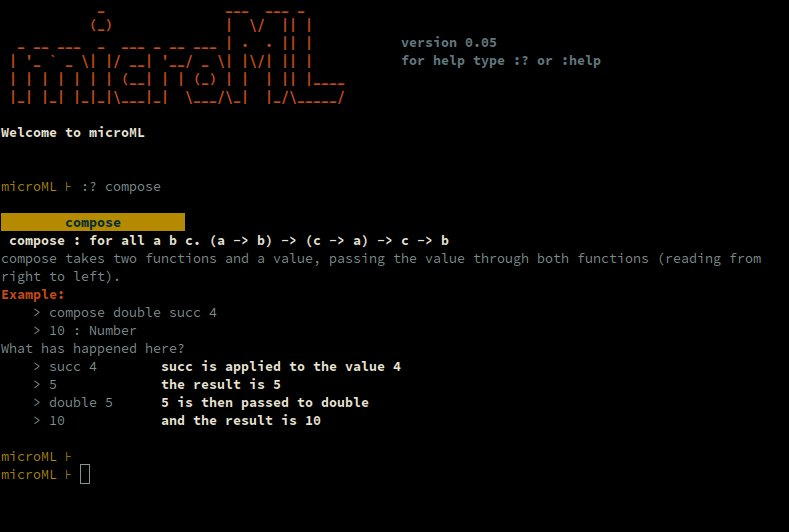
\includegraphics[scale=0.4]{images/comment.jpg}
    {\caption{Comments as seen in the terminal}}
    \label{fig:comments}
\end{SCfigure}

In addition to help regarding function definitions, there is also a glossary of terms for those new
to programming. Terms in the glossary are underlined in the main commentary text.  Another teaching 
tool has been added to the repl environment which the author believes to be unique
is the ability to print the parse tree of an expression within the repl. See figure~\ref{fig:tree}

\begin{SCfigure}
    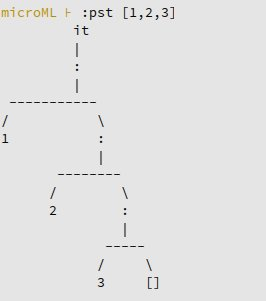
\includegraphics[scale=0.6]{images/tree.jpg}
    {\caption{Parse tree of a simple expression as viewed in the terminal}}
    \label{fig:tree}
\end{SCfigure}

\subsection{Programming Style}
It is the intention of microML to encourage a modularity of design, aiming at function composition
above all. Large, complex functions are to be actively discouraged in favour of smaller, more
`mobile' units. Both Haskell and Miranda support the function composition operator, a single dot.
This is directly taken for the mathematical notion of composition, where it is notated $ f \circ g
$. While it is doubtless more mathematically pure to copy this approach, the expected user of
microML is not a graduate mathematician, but probably only has a GSCE level of maths. MicroML
follows the model of \textbf{Elixir} with its left-to-right \textit{pipe} operator $ |> $. However
microML prefers the notation $ >> $ as being more explicitly about direction and movement.

\section{Implementation}
MicroML is written in Haskell throughout. However it should be stated that this is not the pure
Haskell of the 2010 report, but makes use of a number of extremely useful extensions provided by
the Glasgow Haskell Compiler, GHC.\ This unfortunately does limit the portability of microML, 
but it would be reasonable to say the GHC has largely become the `de facto' Haskell implementation, moving the
language as a whole more in the direction of the Python model, which is defined by CPython, 
rather than a formal document description.

In addition to the main program, there is also a simple vim plugin with syntax highlighting and
comment folding and a primitive autocomplete, which makes editing microML in the editor a slightly more pleasant experience.
Granted, it is a little at odds with the stated objective of microML, which is ease of use and
suitability for beginners, to promote vim as \textit{editor of choice} but this was largely
convenience for the author whose preferred editor is \textbf{neovim}, an ambitious fork of
vim.\footnote{\url{https://neovim.io/}} 

External dependencies to the main program are deliberately few. An experimental JIT compiler makes
use of LLVM\footnote{\url{http://llvm.org/}} with the associated Haskell
bindings\footnote{Unfortunately the bindings are still only for LLVM 3.5, whereas the upstream
version is now 3.8. For this, and other reasons to be discusses, the JIT compiler was abandoned for
this first microML deliverable.}. The compiler also makes optional use of \textbf{clang-format}, a
command line utility available with \textbf{clang}\footnote{\url{http://clang.llvm.org/}} for formatting 
the generated C++ code. The graphics program \textbf{graphviz} is also used (again optionally) for 
producing \textit{png} files of a program's callgraph. 

Handling state in Haskell is by no means trivial, and does not allow for easy prototyping. One needs
to understand exactly how to structure a solution to a problem before embarking on development,
otherwise one risks having to rewrite large sections of code when it becomes apparent that a
particular function needs to reside inside a particular monad, and does not. For example it is not
possible to trivially wrap a function in a \textit{try / except} clause as one would in Python.
Anything which might through an exception needs to be inside the ExceptT monad transformer. The type
checker will reject anything else. This can be sidestepped to a certain extent by throwing an
unchecked \textbf{error}\footnote{a wrapper around the prelude library function \textbf{undefined}},
but such an error kills the runtime system, crashing the program.\footnote{mgrabmueller was
invaluable for understanding the monad transformer abstraction.}

To successfully combine state with error handling it is necessary to `string together' various monad
transformers over a base monad type. While this is an elegant solution and makes writing pure code
easier, it is by no means obvious how to create these initial `stacks' of monads. The advantage
however is that, once the complexity of stack construction has been overcome, this complexity is
`locked away' within one or two data types and functions, allowing the programmer essentially to
forget about state management and error handling details. 

\subsection{Project Structure}
Every effort was made to organize the source code in a logical and consistent manner, such that
another programmer should, without great difficulty.
\dirtree{%
.1 microML.
.2 docs.
.2 src.
.3 Compiler.
.3 Jit.
.3 Libs.
.3 Main.hs.
.3 MicroML.
.4 Typing.
.3 Repl
.2 test.
.3 compiler.
.2 utils.
.3 vim-mmlFold.
.3 mml.vim.
.2 microML.cabal.
.2 stack.yaml.
}

\chapter{Testing}

Software testing is a vital part of any seriously intended development project. Only an arrogant
programmer, or one of little experience (often the two go together) would claim that a function or
module had been written without mistakes, or that all edge cases had been properly handled. It is
difficult for a human to be ruthlessly systematic: precisely the approach that testing needs, and
precisely that which a computer does with ease. Thankfully Haskell has a number of powerful testing
frameworks, making the writing of unit tests especially simple. Both \textit{Cabal} and
\textit{Stack} support integrated testing, making the process of running tests and building trivial.

There are four generally recognized levels of software testing. Unit testing is the examination of
individual methods or functions to ascertain that they behave as expected under a variety of
conditions. This time of testing is best conducted during software development, in concert with the
writing of the actual executable software. Integration testing ensures that individual modules (or
classes) work together as expected. This is one level of abstraction higher than unit-testing.
System testing looks at the functioning of the entire system, and finally acceptance testing sees
whether the end product will be suitable to the client. 

The Hspec\footnote{\url{https://hspec.github.io/}} package focuses primarily on unit testing of
Haskell functions. Real \textit{TDD} would have seen tests written in parallel with production code.
Due to the lack of experience the author had with Haskell at the beginning of the product, this was
not the development method deployed as it would have been too heavy a cognitive burden in addition
to wrestling with various problems of type, state and program structure. Unit tests were written
after the fact, and, at time of writing, do not yet have full coverage of source code.

To run tests while building it is necessary simply to entire the command `stack test' in the
terminal, which is equivalent to building and testing the software.

Testing the ability of the compiler to produce C++ code involved the addition of integration tests
to the Hspec framework. These are handled separately in the form of multiple small \textit{mml}
files. A simple bash script runs each file individually through the microML compiler. At time of
writing, the compiler does not yet successfully pass all of these integration tests. More work needs
to be done before the compiler can seriously be considered to be `fit for purpose'. The script must
be run from the utils folders of the project.

\chapter{Conclusions and Project Evaluation}

\section{Achievements}
Not written yet

\section{Evaluation}
Not written yet

\section{Future Work}
While the basic core of the language is largely complete (at least in the repl environment) a great
deal of work remains to be done on the compiler and making the language more usable as an educational
tool. As a number of features were included in an unfortunately \textit{ad hoc} manner, integration
is not as tight as might be desired. An obvious case of this is the existence of two separate
parsers, one for mml source code, and another for documentation. This has resulted in a rather
fragile relationship between the two, and an over-sensitivity to context (especially around the
existence of unanticipated whitespace) and code duplication in the Repl.Repl module. It also entails
two passes over a source file, which is wasteful of computer resources and time. A future iteration
would seek to unite these into one, more robust parser. Regarding the parser, it might also be a
possibility to make it indentation sensitive. This could result in more readable source files for
students. However, one of the stated aims of microML is to encourage piping of small functions (in
the manner of the unix pipe) rather than building large functions. An indentation sensitive parser
might actively encourage the growth of function complexity. Further investigation would be required
before a definitive decision could be reached.

The present approach to C++ compilation, while valid as a proof of concept, is perhaps not robust
enough to allow for genuine expansion to the level of complexity which might be required of it.
Alternative, better, strategies would involve direct translation of the microML AST to the C++ AST,
enabling the compiler to perform optimisations. Apart from checking the validity of the source file,
the compiler is unable to conduct optimisation routines. Time has been the single greatest factor in
limiting the efficacy of the compiler element of the project. There is a library for the manipulation
of C code in Haskell\footnote{\url{https://hackage.haskell.org/package/language-c}} but there is
nothing specifically for C++. Either the existing library would have  to be modified to allow for
class manipulation and the micro:bit's \textit{managed types} or a new library would have to
written. This is far beyond the scope of the present project, but would seem to be a necessary step
to render the compiler a more industry standard product.

Related to the compiler is the issue of \textit{memory management} on the micro:bit. The API already
exposes a number of managed types which do not require manual freeing, but microML supports closures
and also could be made to support \textit{continuation passing style}, both of which would need to
claim space on the heap and therefore need freeing at some point. A simple \textit{mark \& sweep}
garbage collector is used by microPython. The memory management process for the JavaScript
implementation is not open source. Experiments with microPython have revealed that the garbage
collector takes too much of the available memory for itself. On such a constrained system this can
lead to problems when attempting to use the inbuilt censors or bluetooth. An alternative might be
the use of a \textit{region inference algorithm}\cite{Tofte:2004:RRM:993034.993040}. Work on
MLKit\footnote{\url{http://www.elsman.com/mlkit/}} has shown that region inference memory management
can, at least sometimes, at as a realistic replacement to garbage collection. In a system where
programs are expected to be relatively uncomplicated, such as on the micro:bit, this might be an
ideal `fit'.

Of features missing from the language definition itself, the most obvious omissions are
\textbf{pattern matching} and \textbf{algebraic data types}. The absence of ADTs has already been
discussed, but there presence would be most useful for writing of standard library modules. Without
ADTs the creation of new data structures, while possible, is far more difficult than need be.
Pattern matching is largely syntactic sugar for nested \textit{if --- else if} clauses, and indeed
is desugared in Haskell to nested case statements. A student using microML can simply write such
things themselves, but the ubiquity of pattern matching syntax suggests that it ought to be included
in the language at some point, even if it cannot be regarded as a \textit{primitive} of the
functional style. 

The type inference system is compliant with \textit{System F}. While this is not the most demanding
of type environments within which to work, it might still be too rigid for students with no
programming experience at all, and represent a barrier to entry. Future work might examine the
possibility of \textit{delaying}, or proroguing type checking until the student has fleshed out an
approximate solution to a problem\cite{Afshari:2012:LPP:2384592.2384595}. Type-checking then
becoming an interactive tool for improving software, rather than an overly tight straitjacket it can
seem for those not used to moving within such constraints.

If such a prorogued system could be implemented, then it might be possible to `climb the lambda
cube' as it were. A student could first program dynamically, with duck typing in the manner of
Python, then refine the program to be compliant with System F. It might therefore also be possible
to increase program safety and security by then introducing elements of dependent types where
appropriate. This incremental approach to static typing could encourage students to work with the
type system rather than feel they are fighting it. Even a partially dependently-typed program could
result in a number of possible compiler optimisations and greater runtime safety.

\bibliography{bibliography}{}
\bibliographystyle{plain}

\end{document}
